\newpage
\section{Durchführung}
\label{sec:Durchführung}

\subsection{Versuchsaufbau}
\label{sec:Versuchsaufbau}

In Abbildung \ref{fig:SchemVersuchsaufbau} ist das Prinzip des verwendeten
Versuchsaufbaus dargestellt.
\begin{figure}
  \centering
  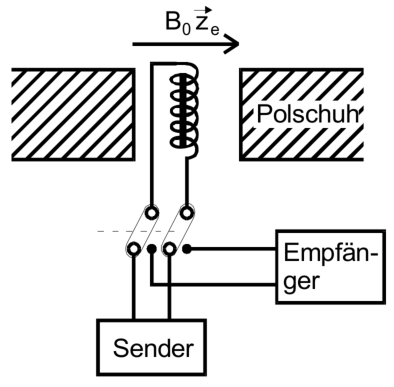
\includegraphics[width=.4\textwidth]{images/versuchsaufbau-schema.pdf}
  \caption{Prinzip des Versuchsaufbaus \cite[7]{anleitung}.}
  \label{fig:SchemVersuchsaufbau}
\end{figure}
Die Probe befindet sich innerhalb einer Spule, die wiederum senkrecht zu einem
Elektromagneten ausgerichtet ist.
Der Elektromagnet bewirkt ein konstantes und möglichst homogenes Magnetfeld $\vec{B}_0$,
während innerhalb der Spule mittels hochfrequenter Ströme ein weiteres
Magnetfeld $\vec{B}_1$ hinzu geschaltet werden kann.
Ein Sender speist diesen hochfrequenten Strom in die Spule und ein Empfänger
misst das Induktionssignal aufgrund der Präzession der Magnetisierung
in der $\vec{x} \vec{y}$-Ebene.

Als Versuchsaufbau wurde eine Teachspin-Apparatur wie in Abbildung \ref{fig:Teachspin}
dargestellt verwendet, dessen NMR-Spektrometer bereits richtig verkabelt ist.
\begin{figure}
  \centering
  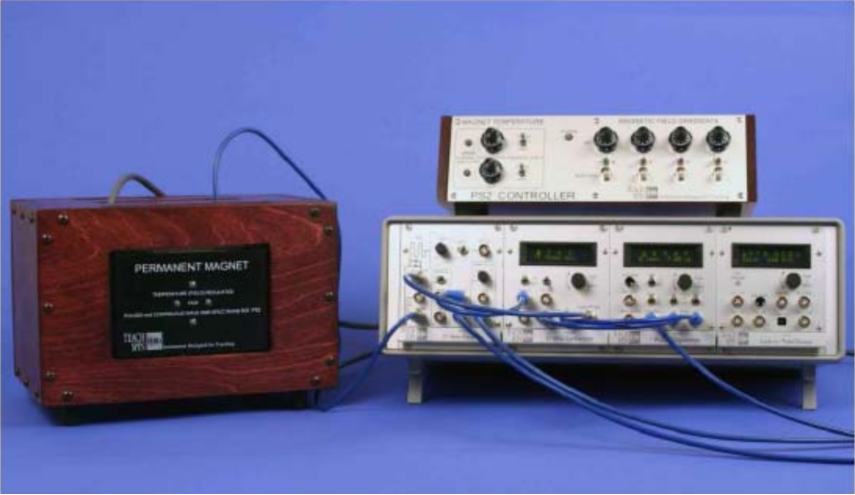
\includegraphics[width=.7\textwidth]{images/teachspin.pdf}
  \caption{Die Teachspin-Apparatur \cite[17]{anleitung}.}
  \label{fig:Teachspin}
\end{figure}
Vor Beginn der Messung müssen nachfolgend beschriebene Parameter einjustiert werden.
Für diese Justage wird eine Wasserprobe verwendet, die paramagnetische Zentren zur
Verkürzung der Relaxationszeiten enthält.
Somit verkürzt sich die Wartezeit, bis die Magnetisierung nach Abschalten von $\vec{B}_1$
wieder in Gleichgewichtslage ist.

Als Vorbereitung auf die Messungen werden zunächst die Gradientenspulen (Shim-Parameter)
auf die Werte
\begin{equation*}
  x = \num{+0.3} \quad y = \num{-4.5} \quad z = \num{+3.52} \quad Z^2 = \num{-2.65}
\end{equation*}
eingestellt.
Der A-Puls wird auf \SI{2}{\micro\second},
die Frequenz des Senders auf \SI{21.7}{\mega\hertz}
und die Wiederholzeit auf \SI{0.5}{\second} eingestellt.
Nun wird zunächst die Resonanzfrequenz gesucht und der auf dem Oszilloskop
angezeigte FID optimiert.
Ist die Frequenz des Senders nicht auf die Resonanzfrequenz (Larmorfrequenz von Wasser)
eingestellt, zeigen sich Oszillationen im Signalbild.
Dies kann damit verstanden werden, dass das rotierende Koordinatensystem nicht
genau auf die Larmorfrequenz eingestellt wurde und somit das Magnetfeld $\vec{B}_1$
nicht statisch ist.
Die Shim-Parameter bezeichnen die Einstellung zwischen den Gradientenspulen des
Magneten, die so eingestellt werden, dass das Magnetfeld möglichst homogen ist.
Im Signal des Oszilloskops spiegelt sich die Homogenität des Magnetfelds durch
einen FID mit langer Zerfallsdauer wieder.
Der A-Puls wird so eingestellt, dass er einen \SI{90}{\degree}-Impuls darstellt.
Schließlich muss die Wiederholzeit P mindestens $2 \tau$ betragen, um die
Antwort des Systems abzuwarten.

Für die eigentlichen Messungen wird nun die Wasserprobe mit den paramagnetischen
Zentren gegen eine Probe ohne Zentren ausgetauscht.
Im Anschluss müssen die oben einjustierten Parameter nicht neu justiert werden.
Die Paramagnetischen Zentren oder auch andere Verunreinigungen haben ein anderes
gyromagnetisches Verhältnis als das betrachtete Wasser, sodass
die Senderfrequenz nicht resonant auf diese Materialien eingestellt sind.


\subsection{Messung von \texorpdfstring{$T_1$}{T1}}
\label{sec:DurchT1}

Die Pulslänge B wird auf die justierte Zeit des \SI{90}{\degree}-Impulses
eingestellt und die Pulslänge A auf die doppelte Zeitspanne.
Hinter dem \SI{180}{\degree}-Impuls darf kein merklicher FID auftreten.
Vermessen wird die Höhe des am \SI{90}{\degree}-Impulses auftretenden
Signals in Abhängigkeit vom Pulsabstand $\tau$ mit Hilfe des Oszilloskops.


\subsection{Messung von \texorpdfstring{$T_2$}{T2}}
\label{sec:DurchT2}

Die Pulslängen A und B der vorherigen Messung werden vertauscht und die Anzahl an
\SI{180}{\degree}-Impulsen sinnvoll eingestellt.
Zunächst wird das in Abbildung \ref{fig:Carr-Purcell-Methode} dargestellte
Bild des Signalverrlaufs am Oszilloskop reproduziert und als Foto gespeichert.
Durch Umlegen des Schalters \texttt{MG} kann im Anschluss auf die MGM gewechselt werden.
Hier ist die zeitliche Abnahme der Echoamplituden deutlich geringer und es
werden so viele Wiederholungen eingestellt, dass die Signalamplitude auf ein Drittel
der ursprünglichen Amplitude abfällt.
Das erhaltene Oszilloskopbild wird als Bild und als Ascii-Datei auf einem USB-Stick
gespeichert.
Nach Abschnitt \ref{sec:DiffusionTheo} muss $T_2$ klein gegen $T_\text{D}$ sein.
Dies ist erfüllt, wenn bei Variation von $\tau$ keine Veränderung im Abklingverhalten
der Spin-Echoamplitude erkennbar ist.


\subsection{Messung der Diffusionskonstanten}
\label{sec:DurchDiffusion}

Die Echoamplitude wird in Abhängigkeit der Zeit $\tau$ vermessen.
Leider ist der Feldgradient $G$ nicht bekannt, sodass ein künstlicher Gradient
in die $\vec{z}$-Richtung eingebaut wird. Dazu werden die Gradientenspulen maximal
weit von der justierten Einstellung für ein homogenes Magnetfeld verstellt.
Der nun erhaltene Gradient lässt sich aus der Halbwertsbreite $t_{\sfrac{1}{2}}$
bestimmen, die mit Hilfe des Oszilloskops bestimmt werden kann.
